\documentclass{llncs}


\usepackage{hyperref}
\usepackage{graphicx}
\usepackage{multirow}
\usepackage[misc,geometry]{ifsym}

\usepackage{amsmath}
\usepackage{enumitem}
%\usepackage{amsfonts}
%\usepackage{amssymb}
%\usepackage{epstopdf}
%\usepackage{epsfig}
\usepackage[T2A]{fontenc}
\usepackage[utf8x]{inputenc}
\usepackage[russian,english]{babel}

\begin{document}

\mainmatter 

\title{A Global Optimization Algorithm for Non-Convex Constrained Mixed-Integer Problems}
\author{Victor Gergel \and Konstantin Barkalov \and Ilya Lebedev %\Letter 
\\
\email{konstantin.barkalov@itmm.unn.ru}}

\institute{
Lobachevsky State University of Nizhni Novgorod, Nizhni Novgorod, Russia
}

\maketitle

\begin{abstract}
\Russian
В работе рассматриваются mixed-integer global optimization problems. Предложен новый детерминированный алгоритм для решения задач данного класса, основанный на information-statistical approach к решению задач непрерывной глобальной оптимизации. Проведено сравнение данного алгоритма с известными аналогами, показывающее эффективность разработанного подхода. Устойчивая работа алгоритма подтверждена также решением серии из нескольких сотен mixed-integer global optimization problems. 

\keywords global optimization, non-convex constraints, mixed-integer problems.

\end{abstract}

\section{Introduction}\label{sec:intro}
\Russian
В работе рассматриваются global optimization problems и методы их решения. Задачи глобальной оптимизации обладают значительной вычислительной трудоемкостью, т.к. глобальный оптимум является интегральной характеристикой решаемой задачи и требует исследования всей области поиска. Как результат, поиск глобального оптимума сводится к построению некоторого покрытия (вообще говоря, неравномерного) в области параметров. Особый интерес представляют задачи, в которых часть параметров может принимать лишь целочисленные значения (mixed-integer global optimization problems), т.к. для них сложнее построить оценки оптимума по сравнению с непрерывными задачами.

Методам решения mixed-integer problems посвящена обширная литература (см., например, обзоры \cite{Burer,Boukouvala}). Известные детерминированные методы решения задач данного класса основаны, как правило, на подходах Branch-and-Bound or Branch-and-Reduce. Также известен ряд метаэвристических и генетических алгоритмов, так или иначе основанных на идеях случайного поиска.

В данной работе нами предложен новый детерминированный метод решения mixed-integer problems, основанный на information-statistical approach к решению задач глобальной оптимизации \cite{Strongin2000,Strongin2013}. Текст статьи, отражающей предварительные результаты исследования, построен следующим образом. Вначале рассмотрен подход к решению задач с непрерывными параметрами, затем предложено его обобщение для mixed-integer problems. В финальном разделе приведены результаты сравнения предложенного метода с известными аналогами.

\section{Global search algorithm and dimension reduction}

Let us consider a multiextremal optimization problem in the form
\begin{gather}\label{problem}
\varphi(y^\ast)=\min{\left\{\varphi(y):y\in D, \; g_i(y)\leq 0, \; 1 \leq i \leq m\right\}},\\
D=\left\{y\in R^N: a_i\leq y_i \leq b_i, 1\leq i \leq N\right\}.\nonumber
\end{gather}
Suppose, that the objective function $\varphi(y)$ (henceforth denoted by $g_{m+1}(y)$) and
the left-hand sides $g_i(y), \; 1\leq i \leq m$, of the constraints satisfy the Lipschitz condition
\[ 
\left|g_i(y')-g_i (y'')\right| \leq L_i \left\|y'-y'' \right\|, \; y',y''\in D, \; 1\leq i \leq m+1, 
\]
with constants $L_i, \; 1 \leq i \leq m+1$, respectively,  and may be multiextremal.

Using a continuous single-valued mapping $y(x)$  (Peano-type space-filling curve) of the interval $[0,1]$ onto $D$, a multidimensional problem (\ref{problem}) can be reduced to a one-dimensional problem
\begin{equation}\label{problem1}
\varphi(y(x^\ast))=\min \left\{\varphi(y(x)): x \in [0,1], \; g_i(y(x))\leq 0, \; 1 \leq i \leq m\right\}.
\end{equation}
The reduction of dimensionality matches the multidimensional problem with a Lipschitzian objective function and constraints with a one-dimensional problem where the respective functions satisfy the uniform H\"older condition (see \cite{Strongin2000}).

%Проверить
An efficient global search algorithm (GSA) for solving constrained optimization problem (\ref{problem1}) was developed at University of Nizhni Novgorod. A detailed description of the algorithm and the corresponding convergence theory are presented in \cite{Strongin2000}.

\section{Global search algorithm for mixed-integer problems}

\Russian
Рассмотрим теперь способ адаптации GSA для решения mixed-integer global optimization problems 

\begin{gather}\label{problem_i}
\min{\left\{ g_{m+1}(y):y\in D, \; g_i(y)\leq 0, \; 1 \leq i \leq m\right\}},\\
D=\left\{a_i\leq y_i \leq b_i, \; 1\leq i \leq N, \; y_j \in Z, \; j \in J, \; y_i \in R, \; i \notin J \right\}.\nonumber
\end{gather}

На основе задачи (\ref{problem_i}) сформируем множество задач 
\begin{gather}\label{problem_is}
\min{\left\{ g_{m+1}^s(y):y\in D^s, \; g_i^s(y)\leq 0, \; 1 \leq i \leq m\right\}},\\
D^s=\left\{ a_i\leq y_i \leq b_i, \;  y_i \in R, \; i \notin J \right\}, \; s\in\{1,...,S\},\nonumber 
\end{gather}
каждая из которых соответствует исходной задаче (\ref{problem_i}) с фиксированным набором целочисленных параметров. Число задач $S$ будет соответствовать числу возможных комбинаций целочисленных параметров.

Используя схему редукции размерности с помощью развертки $y(x)$ на основе множества задач (\ref{problem_is}) можно составить единую задачу
\begin{equation}\label{problem_is1}
\min \left\{g_{m+1}^s(y(x)): x \in [0,S], \; g_i^s(y^s(x)) \leq 0, \; 1 \leq i \leq m\right\},
\end{equation}
где отображение $y^s(x)$  формируется на основе исходной развертки $y(x)$ следующим образом
\[
y^s(x)=y(x-s), \; x\in[s-1,s],\; s\in\{1,...,S\}.
\]
Функции $g_i^s(y^s(x))$ могут иметь разрывы в точках $s\in \{1,...,S-1\}$, поэтому данные точки рассматриваются как выколотые, значение objective function and constraints в них не определено.

Для иллюстрации на Fig. \ref{fig:1}  изображены графики функций, соответствующих задаче с одним непрерывным и одним бинарным параметром.

\begin{figure}[ht]
    \centering
    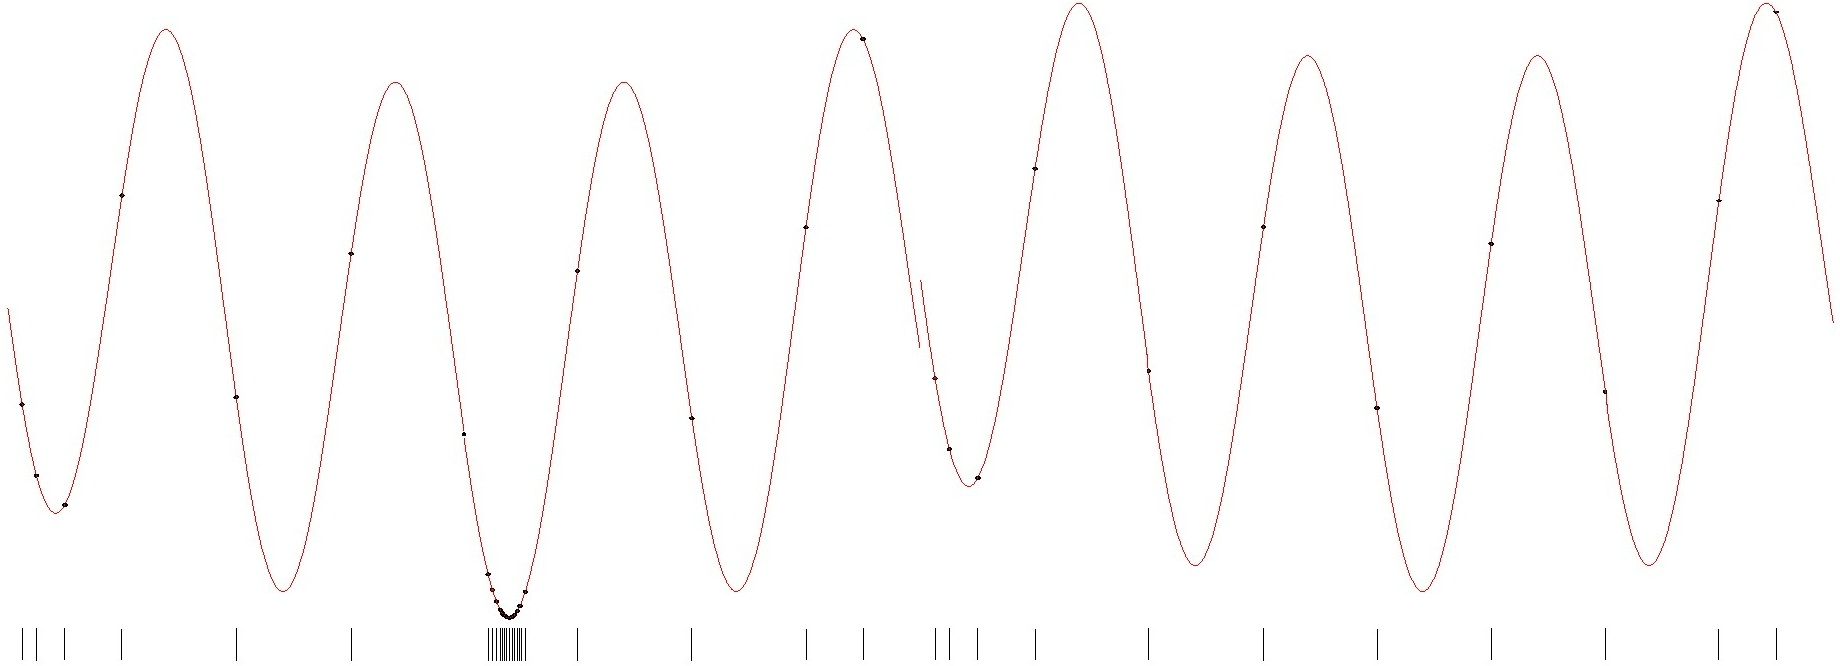
\includegraphics[width=0.7\textwidth]{fig1.jpg}
    \caption{Mixed-integer global optimization problem}
    \label{fig:1}
\end{figure}

Применяя к решению задачи (\ref{problem_is1}) алгоритм глобального поиска, мы найдем решение задачи (\ref{problem_i}). При этом основная часть испытаний будет проведена в $s$-й подзадаче, решение которой соответствует решению исходной задачи (\ref{problem_i}). В остальных подзадачах будет проведена лишь незначительная часть испытаний, т.к. решения данных подзадач являются локально-оптимальными по отношению к решению $s$-й подзадачи. Сказанное подтверждается Fig. \ref{fig:1}, где штрихами обозначены точки испытаний, выполненных при решении данной задачи.

Таким образом, мы сформировали Mixed-Integer Global Search Algorithm (MIGSA), основанный на сведении задачи MINLP путем к задаче NLP. Можно доказать, что условия сходимости данного алгоритма будут следовать из условий сходимости его прототипа (GSA).

\section{Results of experiments}

\Russian
Проведем сравнение предложенного метода MIGSA с genetic algorithm for solving mixed-integer optimization problems, реализованным в Matlab Global Optimization Toolbox. В Table \ref{tab:1} приведено число испытаний, потребовавшееся для решения известных тестовых mixed-integer problems данными методами. Для обоих методов была использована одинаковая точность поиска решения $10^{-2}$. Все вычислительные эксперименты были проведены на компьютере с процессором Intel Core i5-7300 2.5 GHz и 8 Gb RAM под управлением MS Windows 10. Результаты экспериментов показывают превосходство метода MIGSA как по числу итераций, так и по времени работы.

\begin{table}
	\caption{Сравнение эффективности методов MIGSA и GA}
	\label{tab:1}
	\center
	\begin{tabular}{cccccc}
		\hline\noalign{\smallskip}
	\multirow{2}{*}{Test problem}	 & \multicolumn{2}{c}{ GA } & & \multicolumn{2}{c}{MIGSA} \\
		\noalign{\smallskip} \cline{2-3} \cline{5-6} \noalign{\smallskip}
		 & $k$ & $t$ & & $k$ & $t$  \\
		\noalign{\smallskip} \hline \noalign{\smallskip}
		 Problem 2 \cite{Floudas}&	481 &	0.0601 & &	417 &	0.04 \\
%		 Problem 3 \cite{Floudas}& 	1821 &	0.1130 & & 3324 &	0.107 \\
		 Problem 6 \cite{Floudas}&	641 &	0.0510 & &	118 &	0.001 \\
		 Problem 1 \cite{Deep}   &	481 &	0.1378 & &	66 &	0.0007 \\
		 Problem 2 \cite{Deep}   &	481 &	0.0473 & &	57 &	0.0006 \\
		 Problem 7 \cite{Deep}   &	841 &	0.0736 & & 372	 &	0.017 \\
		\noalign{\smallskip}\hline
	\end{tabular}
\end{table}

Для демонстрации надежности метода MIGSA нами были решены четыре серии по 100 многоэкстремальных mixed-integer problems, построенных на основе модифицированных классов задач Simple и Hard, сгенерированных генератором GKLS \cite{Gaviano}. 
Данный генератор многоэкстремальных функций часто используется для исследования алгоритмов непрерывной оптимизации \cite{Paulavicius2014,SergeyevKvasov2015,Lebedev2015,Gergel2015}.
 В сгенерированных нами задачах было 5 целочисленных и 3 непрерывных параметра. Точность поиска решения равнялась $10^{-2}$ по координате. Все задачи из серии были успешно решены , при этом для решения задач на основе класса Simple потребовалось среднем 11988 trials, а для решения задач на основе класса Hard -- 24750 trials.


\textbf{Acknowledgments}. This study was supported by the Russian Science Foundation, project No 16-11-10150.

\begin{thebibliography}{10}

\bibitem{Burer}
Burer, S., Letchford, A.N.: Non-convex mixed-integer nonlinear programming: A survey. Surveys in Operations Research and Management Science \textbf{17}, 97--106 (2012) 

\bibitem{Boukouvala}
Boukouvala, F., Misener, R., Floudas, C.A.: Global optimization advances in Mixed-Integer Nonlinear Programming, MINLP, and Constrained Derivative-Free Optimization, CDFO. European Journal of Operational Research \textbf{252}, 701--727 (2016) 

\bibitem{Strongin2000}
Strongin, R.G., Sergeyev, Y.D.: Global Optimization with Non-Convex Constraints. Sequential and Parallel Algorithms. Kluwer Academic Publishers, Dordrecht (2000) %; DOI: 10.1007/978-1-4615-4677-1

\bibitem{Strongin2013}
Sergeyev, Ya.D., Strongin, R.G., Lera, D.: Introduction to global optimization exploiting space-filling curves. Springer (2013) %;  DOI: 10.1007/978-1-4614-8042-6

\bibitem{Floudas}
Floudas, C.A., Pardalos, P.M.:  Handbook of Test Problems in Local and Global Optimization. Springer (1999)  %; DOI: 10.1007/978-1-4757-3040-1

\bibitem{Deep}
Deep, K., Singh, K. P., Kansal, M.L., Mohan, C.: A real coded genetic algorithm for solving integer and mixed integer optimization problems. Appl. Math. Comput. \textbf{212}(2), 505--518 (2009)

\bibitem{Gaviano}
Gaviano, M., Kvasov, D.E, Lera, D., and Sergeyev, Ya.D.: Software for generation of classes of test functions with known local and global minima for global optimization. ACM Transactions on Mathematical Software \textbf{29}(4), 469--480 (2003)

\bibitem{Paulavicius2014} 
Paulavi\v{c}ius, R., Sergeyev, Y., Kvasov, D., \v{Z}ilinskas, J.: Globally-biased DISIMPL algorithm for expensive global optimization. J. Glob. Optim. \textbf{59}(2-3), 545--567 (2014)

\bibitem{SergeyevKvasov2015} 
Sergeyev, Y.D., Kvasov, D.E.: A deterministic global optimization using smooth diagonal auxiliary functions. Commun. Nonlinear. Sci. Numer. Simulat. \textbf{21}(1-3), 99--111 (2015)

\bibitem{Lebedev2015}
Lebedev, I., Gergel, V.: Heterogeneous Parallel Computations for Solving Global Optimization Problems. Procedia Computer Science \textbf{66}, 53--62 (2015)

\bibitem{Gergel2015}
Gergel, V., Sidorov, S.: A Two-Level Parallel Global Search Algorithm for Solution of Computationally Intensive Multiextremal Optimization Problems. Lecture Notes in Computer Science  \textbf{9251}, 505--515 (2015)


\end{thebibliography}


\end{document}
______________________________________________________________________
